\documentclass{article}

\usepackage{microtype}
\usepackage{graphicx}
\usepackage{subcaption}
\usepackage{booktabs}
\usepackage{hyperref}
\newcommand{\theHalgorithm}{\arabic{algorithm}}
\usepackage{icml2026}
\usepackage{amsmath}
\usepackage{amssymb}
\usepackage{mathtools}
\usepackage{amsthm}
\usepackage[capitalize,noabbrev]{cleveref}

\icmltitlerunning{Mechanistic Interpretability of Source Arbitration in LLMs}

\begin{document}
\twocolumn[
  \icmltitle{Instruction Readers, Not Document Copiers: \\
  Mechanistic Interpretability of Source Arbitration \\
  Across Instruction-Tuned Language Models}

  \begin{icmlauthorlist}
    \icmlauthor{Anonymous}{anon}
  \end{icmlauthorlist}

  \icmlaffiliation{anon}{Anonymous Institution}

  \icmlcorrespondingauthor{Anonymous Author}{anon@domain.com}
  \icmlkeywords{Mechanistic Interpretability, Source Arbitration, RAG, Knowledge Conflict, Language Models}
  \vskip 0.3in
]

\printAffiliationsAndNotice{}

% ============================================================
% ABSTRACT
% ============================================================
\begin{abstract}
When retrieved documents contradict a language model's parametric knowledge, the model must decide whether to follow the supplied context or rely on memory. We study this source-arbitration computation in a controlled factual-conflict benchmark across three instruction-tuned models: Qwen2.5-3B-Instruct, Qwen2.5-1.5B-Instruct, and Gemma-2-2B-IT. Using token-variant-aware scoring with residual-stream patching, attention-head patching, direct logit attribution, attention decomposition, linear probes, activation steering, and cumulative head-set controls, we find that context-override behavior localizes to late layers, typically within the final 8--12\% of model depth. Our central observation is that the most influential heads are not document copiers: they attend primarily to the question/instruction region while assigning negligible attention to document tokens, yet substantially influence whether the model selects the document answer. This supports a mechanistic picture in which earlier layers encode document content into the residual stream, while late-layer heads implement instruction-conditioned source selection. Across the tested models, we observe distinct implementation patterns---concentrated override heads, memory-defense heads, and distributed committee-like heads---suggesting that source arbitration may be a recurring late-layer function with model-specific mechanisms.
\end{abstract}

% ============================================================
% 1. INTRODUCTION
% ============================================================
\section{Introduction}
\label{sec:intro}

Retrieval-augmented generation (RAG) systems augment language models with external documents at inference time~\citep{liu2023lost}. A critical failure mode occurs when retrieved documents contain information conflicting with the model's parametric knowledge. In such cases, the model must \textit{arbitrate} between sources: follow the document (context-adherence) or trust its training (memory-adherence).

Prior work has identified ``context heads'' that preferentially attend to in-context information~\citep{shi2024context,wolfson2025taming,wu2024retrieval}. However, existing studies have three key limitations: (1)~they do not separate \emph{instruction-conditioned} source selection from \emph{autonomous arbitration}; (2)~they implicitly treat context-override as a content-copying operation; and (3)~they analyze single model families.

We address these gaps with three contributions:

\begin{enumerate}
    \item \textbf{Regime separation.} We explicitly distinguish instruction-conditioned selection from ambiguous arbitration, showing they activate overlapping but quantitatively distinct behavioral patterns.
    
    \item \textbf{The instruction-reader finding.} We observe that context-override heads pay negligible attention to the document text. Instead, they attend to the instruction region and write the document answer using representations computed by earlier layers.
    
    \item \textbf{Cross-family taxonomy.} We identify three distinct mechanistic strategies for a similar functional role across two model families, providing suggestive evidence of a recurring late-layer source-arbitration pattern across the tested models.
\end{enumerate}

% ============================================================
% 2. RELATED WORK
% ============================================================
\section{Related Work}
\label{sec:related}

\paragraph{Knowledge conflict in LLMs.}
\citet{longpre2021entity} systematically studied how models handle parametric-contextual conflicts. \citet{chen2022rich} showed larger models are more susceptible to counterfactual context. \citet{jin2024knowledge} analyzed where conflicts are resolved within transformer layers.

\paragraph{Mechanistic interpretability of factual recall.}
The ROME framework~\citep{meng2022rome} identified factual associations in MLP layers. Causal tracing~\citep{meng2023mass} showed factual recall involves localized mid-to-late layer circuits. \citet{geva2023dissecting} dissected recall of factual associations in auto-regressive models.

\paragraph{Context-preference heads.}
\citet{shi2024context} identified attention heads that preferentially attend to in-context information. \citet{wu2024retrieval} found sparse retrieval heads causally responsible for long-context factuality. \citet{wolfson2025taming} proposed interventions to tame conflicts. Our work extends this line by providing a more detailed mechanistic decomposition---not just \emph{which} heads matter, but \emph{what they attend to}, \emph{what they write}, and \emph{how to steer them}.

\paragraph{Activation steering.}
\citet{li2024inference} and \citet{turner2024activation} demonstrated that adding direction vectors to activations can steer model behavior. We apply steering to source arbitration, finding that steering direction \emph{inverts} for memory-defense heads, providing directionally consistent evidence of head polarity.

% ============================================================
% 3. METHODOLOGY
% ============================================================
\section{Methodology}
\label{sec:method}

\subsection{Models and Dataset}

We study three instruction-tuned models spanning two families: Qwen2.5-3B-Instruct and Qwen2.5-1.5B-Instruct~(Qwen family), and Gemma-2-2B-IT~(Google family). Table~\ref{tab:models} summarizes architectures and dataset statistics.

We construct a benchmark of 501 real-world facts across 10 categories, each paired with a plausible counterfactual distractor. Each fact generates prompts under four regimes: \textit{explicit context} (``Based only on the document above\ldots''), \textit{ambiguous conflict} (no source instruction), \textit{explicit memory} (``Using your own knowledge\ldots''), and \textit{naturalistic RAG} (multi-document retrieval style).

\begin{table}[t]
\centering
\resizebox{\columnwidth}{!}{%
\begin{tabular}{lccc}
\toprule
\textbf{Property} & \textbf{Qwen-3B} & \textbf{Qwen-1.5B} & \textbf{Gemma-2B} \\
\midrule
Architecture & Qwen2.5 & Qwen2.5 & Gemma-2 \\
Layers & 36 & 28 & 26 \\
Hidden dim & 2048 & 1536 & 2304 \\
Attn heads & 16 & 12 & 8 \\
\midrule
Single-token valid & 189 & 189 & 243 \\
Matched pairs (explicit) & 133 & 149 & 227 \\
Pair yield & 70.4\% & 78.8\% & 93.4\% \\
\bottomrule
\end{tabular}%
}
\caption{Model architectures and dataset filtering funnel. Gemma's higher yield reflects stronger baseline context-adherence.}
\label{tab:models}
\end{table}


\subsection{Token-Variant-Aware Filtering}

A key methodological contribution is our token-variant-aware filtering. The same entity can tokenize differently depending on context (e.g., ``Paris'' $\to$ \texttt{[Paris]} vs \texttt{[Par, is]}). We enumerate all single-token variants for each answer and restrict causal tracing to facts where both answers have valid single-token representations.

\subsection{Source Preference Score}

We define the \textbf{Source Preference Score} (SPS) as:
\begin{equation}
\text{SPS} = \max_{v \in V_{\text{ctx}}} \log p(v) - \max_{v \in V_{\text{mem}}} \log p(v)
\label{eq:sps}
\end{equation}
where $V_{\text{ctx}}$ and $V_{\text{mem}}$ are sets of valid single-token variants for context and memory answers. SPS~$>$~0 indicates context-adherence.

\subsection{Causal Intervention Pipeline}

We apply six complementary interventions:

\paragraph{1. Residual stream patching.} Replace layer $\ell$'s residual output from the document-present run with the no-document run. Measure $\Delta$SPS.

\paragraph{2. Head patching.} Same as above at individual attention head granularity to isolate specific heads.

\paragraph{3. Direct Logit Attribution (DLA).} Decompose each head's output through the unembedding matrix $W_U$ to measure direct contribution to context vs.\ memory token logits:
\begin{equation}
\text{DLA}_h = h \cdot W_U[\text{ctx}] - h \cdot W_U[\text{mem}]
\end{equation}

\paragraph{4. Attention pattern analysis.} Measure attention distribution across document, question/instruction, and other regions.

\paragraph{5. Linear probing.} Train logistic regression probes on residual stream activations at each layer to predict source choice.

\paragraph{6. Activation steering.} Compute a ``context direction'' vector from attention outputs and add $\alpha \times$ direction during inference to test causal sufficiency~\citep{turner2024activation}.

\paragraph{Sample sizes.} Baseline evaluations (Table~\ref{tab:baselines}) use all single-token-valid facts (189--243 per model). Causal interventions (patching, DLA, attention, steering) subsample 40--60 matched pairs per experiment for computational tractability, with fixed random seed for reproducibility. Table~\ref{tab:models} reports the total matched-pair pool; each causal experiment draws from this pool.

% ============================================================
% 4. RESULTS
% ============================================================
\section{Results}
\label{sec:results}

\subsection{Baseline Source Preference}

\begin{table}[t]
\centering
\resizebox{\columnwidth}{!}{%
\begin{tabular}{lccc}
\toprule
\textbf{Regime} & \textbf{Qwen-3B} & \textbf{Qwen-1.5B} & \textbf{Gemma-2B} \\
\midrule
Explicit context & 86.2\% & 95.8\% & 98.4\% \\
Ambiguous conflict & 87.3\% & 97.9\% & 78.2\% \\
Explicit memory & 66.7\% & 82.0\% & 25.9\% \\
\bottomrule
\end{tabular}%
}
\caption{Baseline context-win rates (\%) across regimes. Gemma shows strong instruction-conditional gating: 98.4\% when instructed to follow context, but only 25.9\% when told to use memory.}
\label{tab:baselines}
\end{table}


Table~\ref{tab:baselines} reveals two key behavioral findings:

\textbf{Finding 1: Instruction-conditional gating in Gemma.} Gemma shows notable regime sensitivity: 98.4\% context-following when instructed, but only 78.2\% without instruction, and 25.9\% when told to use memory. This is consistent with a gating mechanism sensitive to instruction presence and polarity.

\textbf{Finding 2: Non-monotonic scaling in Qwen.} Qwen-1.5B (smaller) is \emph{more} context-compliant than Qwen-3B (larger): 95.8\% vs 86.2\%. This does not follow the common assumption that larger models are more instruction-compliant. One possible explanation is that 3B's stronger parametric knowledge creates greater resistance to context-override.

\subsection{Circuit Localization}

\begin{figure*}[t]
    \centering
    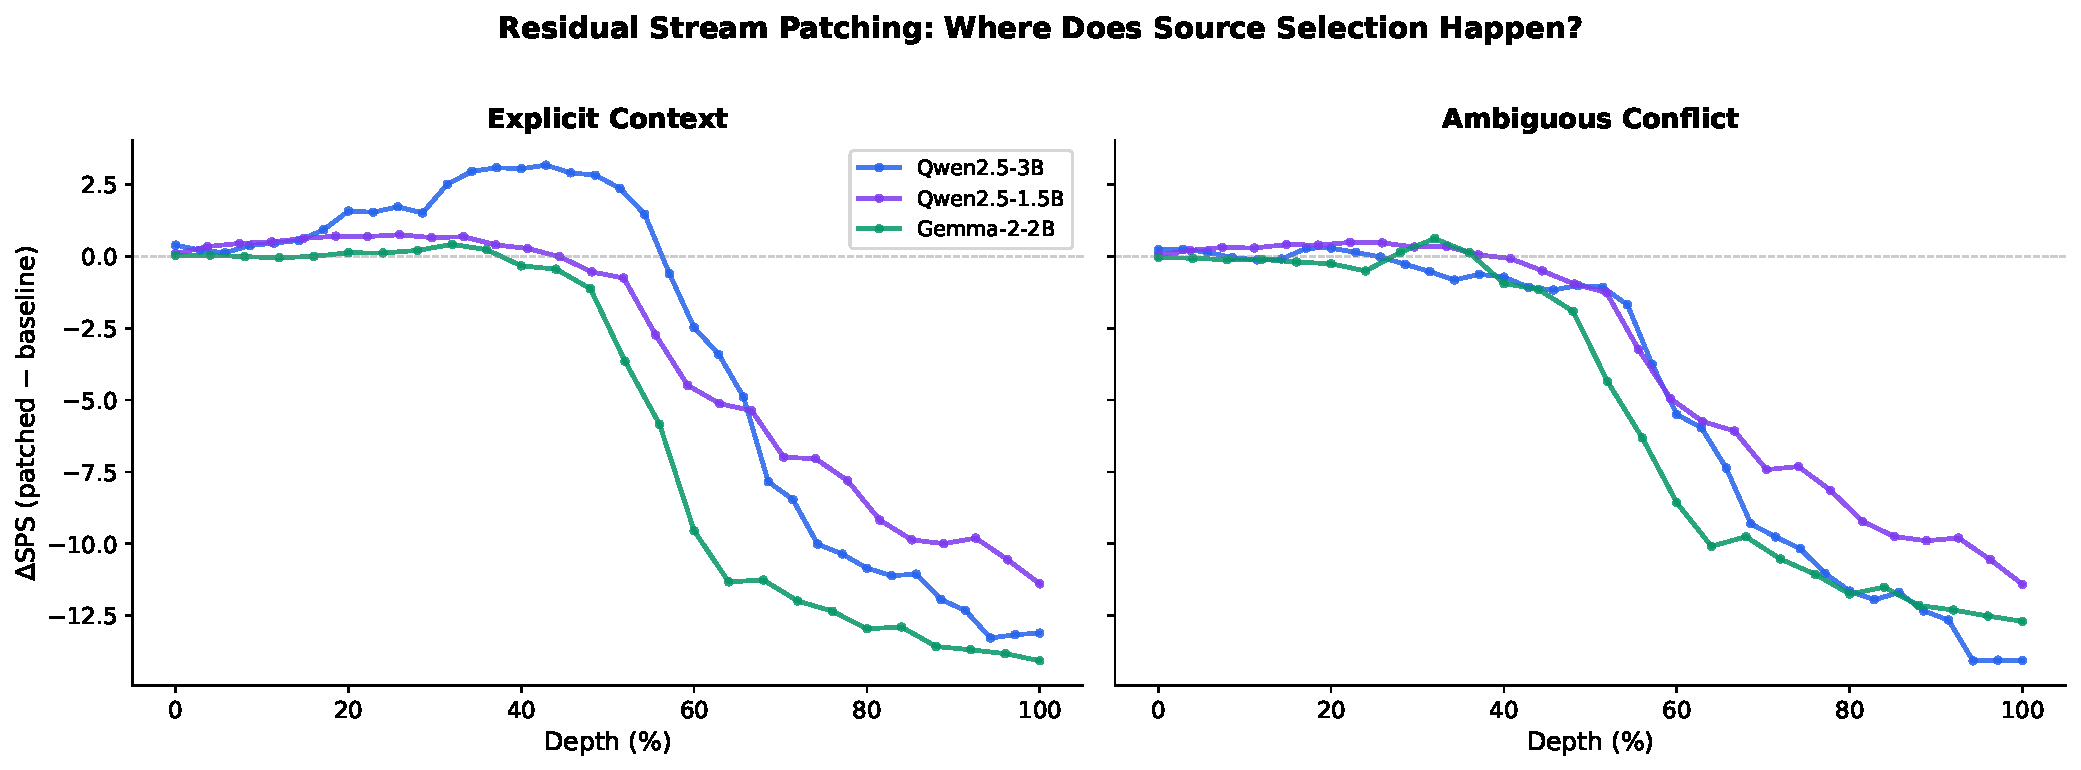
\includegraphics[width=\textwidth]{figures/fig1_residual_patching.pdf}
    \caption{\textbf{Residual Stream Patching.} Layer-wise $\Delta$SPS curves for all three models under explicit context (left) and ambiguous conflict (right) regimes. The first 50\% of layers show near-zero effect; context-override is concentrated in the final 8--12\% of depth.}
    \label{fig:patching}
\end{figure*}

Residual stream patching (Figure~\ref{fig:patching}) reveals a consistent pattern: the first 50--60\% of layers have near-zero $\Delta$SPS, followed by a sharp decline in the final layers.

\begin{table}[t]
\centering
\resizebox{\columnwidth}{!}{%
\begin{tabular}{lccc}
\toprule
\textbf{Metric} & \textbf{Qwen-3B} & \textbf{Qwen-1.5B} & \textbf{Gemma-2B} \\
\midrule
Peak layer & L33 & L27 & L25 \\
Peak depth (\%) & 94.3 & 100.0 & 100.0 \\
Peak $\Delta$SPS & $-13.28$ & $-11.39$ & $-14.07$ \\
\midrule
Top head & L31.H10 & L27.H1 & L22.H1 \\
Top head $\Delta$SPS & $-0.25 \pm 0.13$ & $-0.12 \pm 0.05$ & $-0.25 \pm 0.07$ \\
Sig.\ heads ($|\Delta\text{SPS}|{>}0.1$) & 20 & 7 & 9 \\
\bottomrule
\end{tabular}%
}
\caption{Circuit localization via residual stream and head patching. All models localize context-override to the final 6--12\% of depth. Top head $\Delta$SPS shows 95\% CI margins.}
\label{tab:patching}
\end{table}


\textbf{Finding 3: Universal late-layer localization.} The context-override circuit is localized to the final 6--8\% of model depth across both model families (Table~\ref{tab:patching}). Patching earlier layers produces negligible effects, indicating source-selection is computed \emph{after} semantic processing is complete.

\subsection{Direct Logit Attribution}

\begin{figure*}[t]
    \centering
    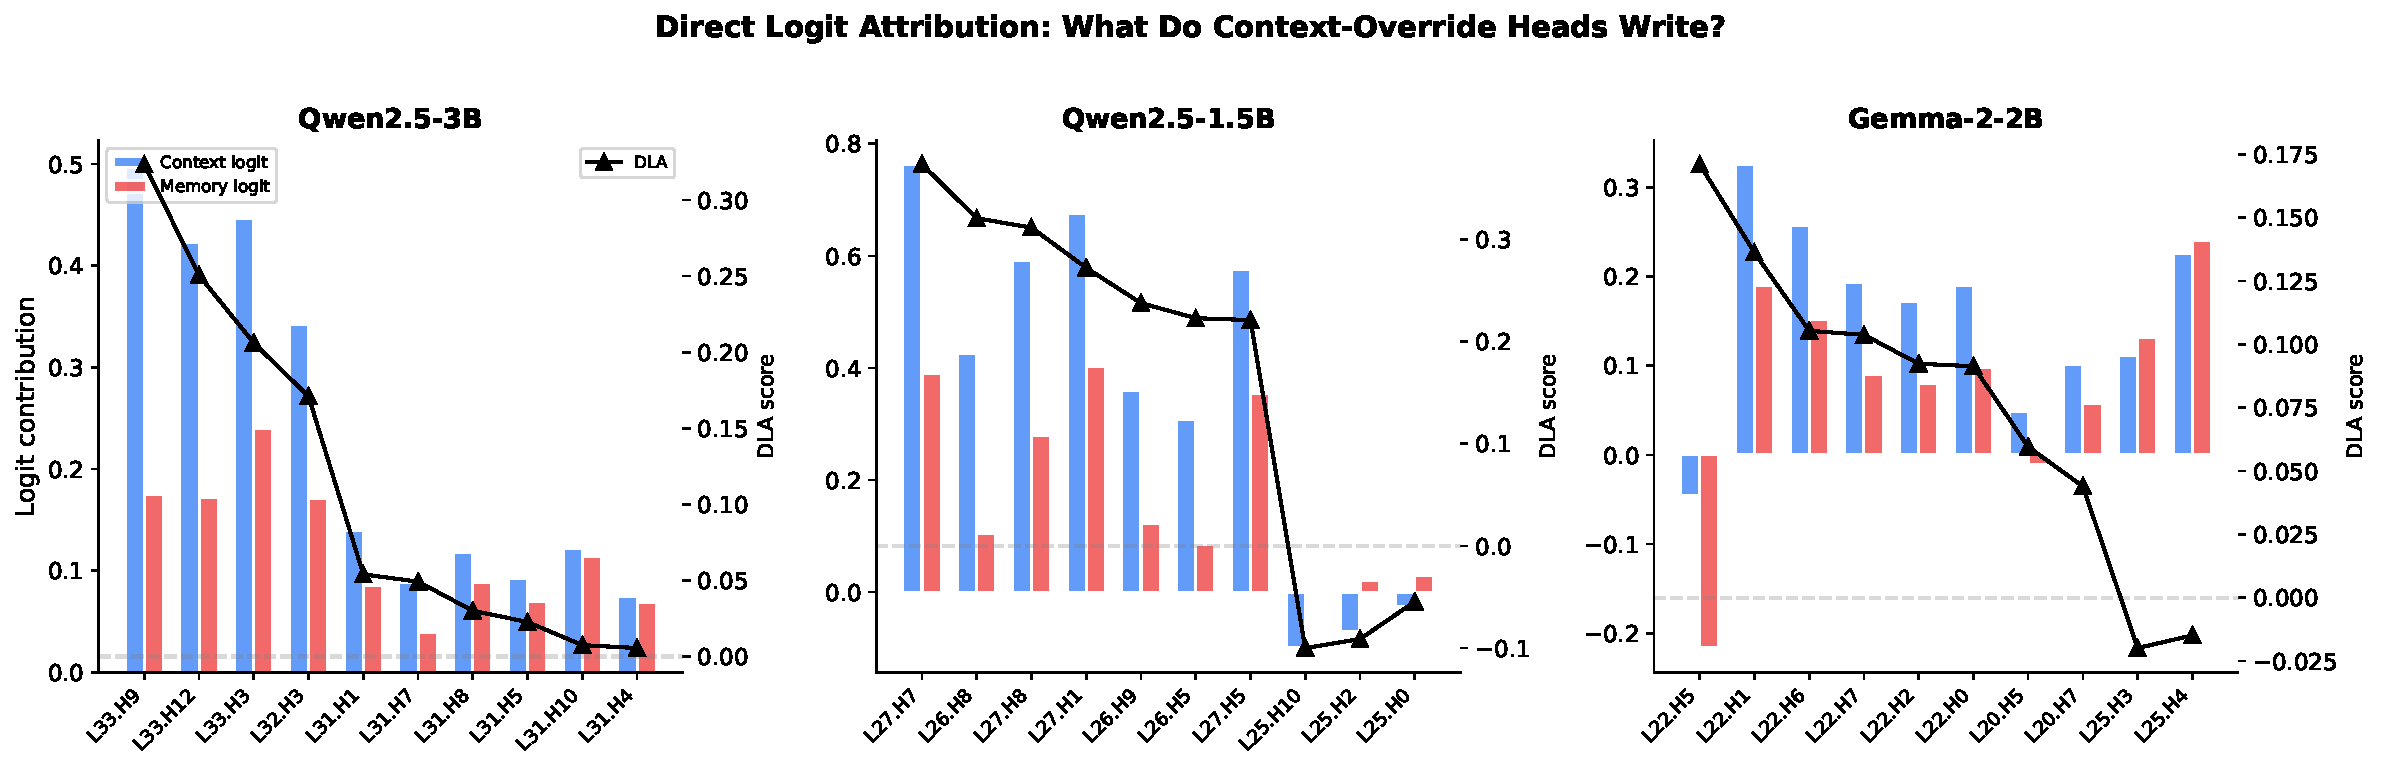
\includegraphics[width=\textwidth]{figures/fig2_dla_heatmap.pdf}
    \caption{\textbf{Direct Logit Attribution.} For each model's top-10 heads, blue bars show context-token logit contribution, red bars show memory-token contribution. The black line shows DLA (context minus memory). Note Qwen-1.5B's rightmost heads with negative DLA (memory-defense heads).}
    \label{fig:dla}
\end{figure*}

\begin{table}[t]
\centering
\resizebox{\columnwidth}{!}{%
\begin{tabular}{lccc}
\toprule
\textbf{Metric} & \textbf{Qwen-3B} & \textbf{Qwen-1.5B} & \textbf{Gemma-2B} \\
\midrule
Top DLA head & L33.H9 & L27.H7 & L22.H5 \\
DLA score & $0.324 \pm 0.11$ & $0.373 \pm 0.16$ & $0.171 \pm 0.06$ \\
Ctx logit & $+0.498$ & $+0.763$ & $-0.046$ \\
Mem logit & $+0.175$ & $+0.390$ & $-0.217$ \\
Neg-DLA heads & 0 & 3 & 2 \\
\midrule
Avg doc attn & 0.0\% & 0.0\% & 0.0\% \\
Avg question attn & 57.6\% & 38.5\% & 24.2\% \\
\bottomrule
\end{tabular}%
}
\caption{Direct Logit Attribution and attention patterns (95\% CI margins for DLA). All models show 0\% document attention---context-override heads read the instruction, not the document.}
\label{tab:dla_attn}
\end{table}


DLA decomposes each head's output through $W_U$ (Figure~\ref{fig:dla}, Table~\ref{tab:dla_attn}):

\textbf{Finding 4: Memory-defense heads in Qwen-1.5B.} While all models' top heads have positive DLA, Qwen-1.5B uniquely contains 3 heads with \emph{negative} DLA---heads that actively write memory-token logits. These ``memory-defense'' heads represent a pull-back mechanism absent in the larger Qwen-3B.

\textbf{Finding 5: Gemma uses differential suppression.} Gemma's top head (L22.H5) has negative logit contributions for \emph{both} tokens, but suppresses memory more ($-0.217$ vs $-0.046$). The net DLA is positive through suppression, not promotion---a qualitatively different strategy from Qwen.

\subsection{The Instruction-Reader Finding}

\begin{figure}[t]
    \centering
    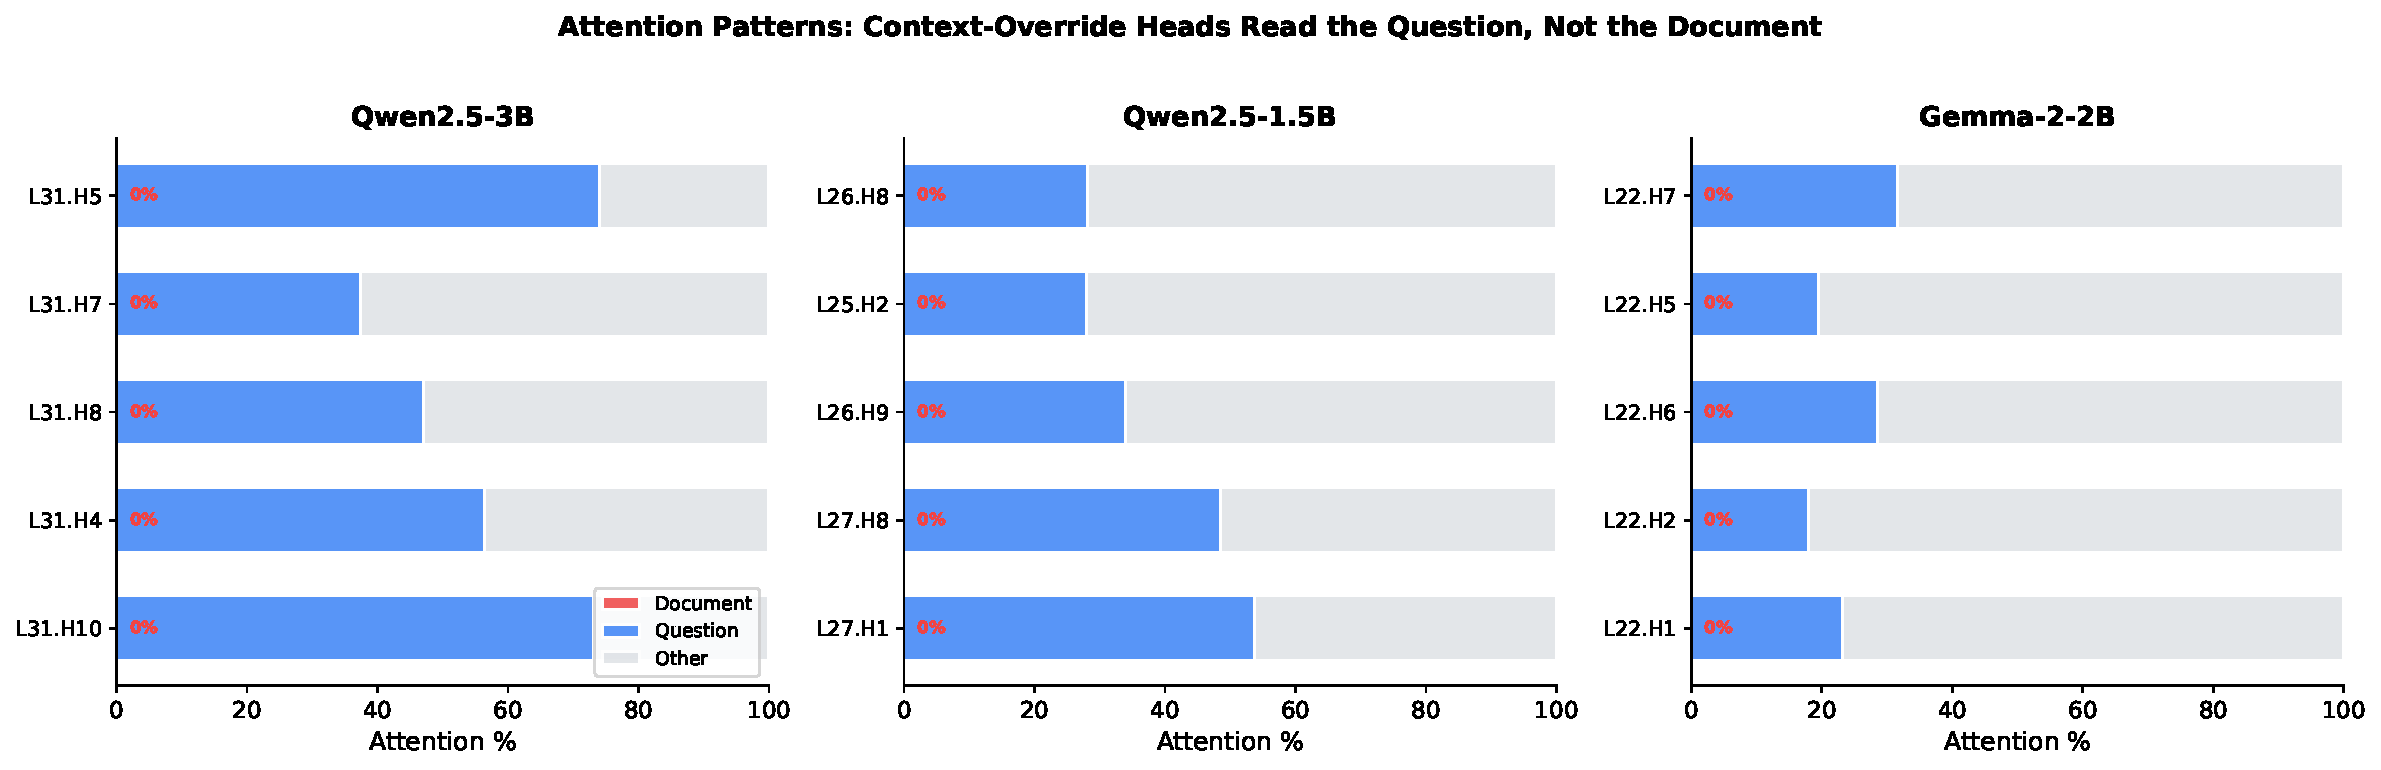
\includegraphics[width=\columnwidth]{figures/fig3_attention_patterns.pdf}
    \caption{\textbf{Attention Patterns.} Context-override heads attend 0\% to the document (red) and 25--57\% to the question/instruction (blue). They are instruction readers, not document copiers.}
    \label{fig:attention}
\end{figure}

Across all three models, context-override heads pay \textbf{negligible attention to the document} (Table~\ref{tab:dla_attn}, Figure~\ref{fig:attention}). Instead, they attend to the question/instruction region (25--57\%).

\textbf{Finding 6: Context-override heads are instruction readers, not document copiers.} This contrasts with the intuitive model of context-override as ``the head reads the document and copies its answer.'' The observed mechanism is:
\begin{enumerate}
    \item \textbf{Early layers} (L0--L20): Process and encode document content into the residual stream.
    \item \textbf{Late-layer heads} (L22--L33): Attend to the \emph{instruction} region, consistent with determining source-selection policy, then write the appropriate answer using document representations already in the residual stream.
\end{enumerate}
The circuit appears to function as an \emph{instruction-conditioned policy executor} rather than a content copier.

\subsection{Probing and Steering}

\begin{figure*}[t]
    \centering
    \begin{subfigure}[b]{0.48\textwidth}
        \centering
        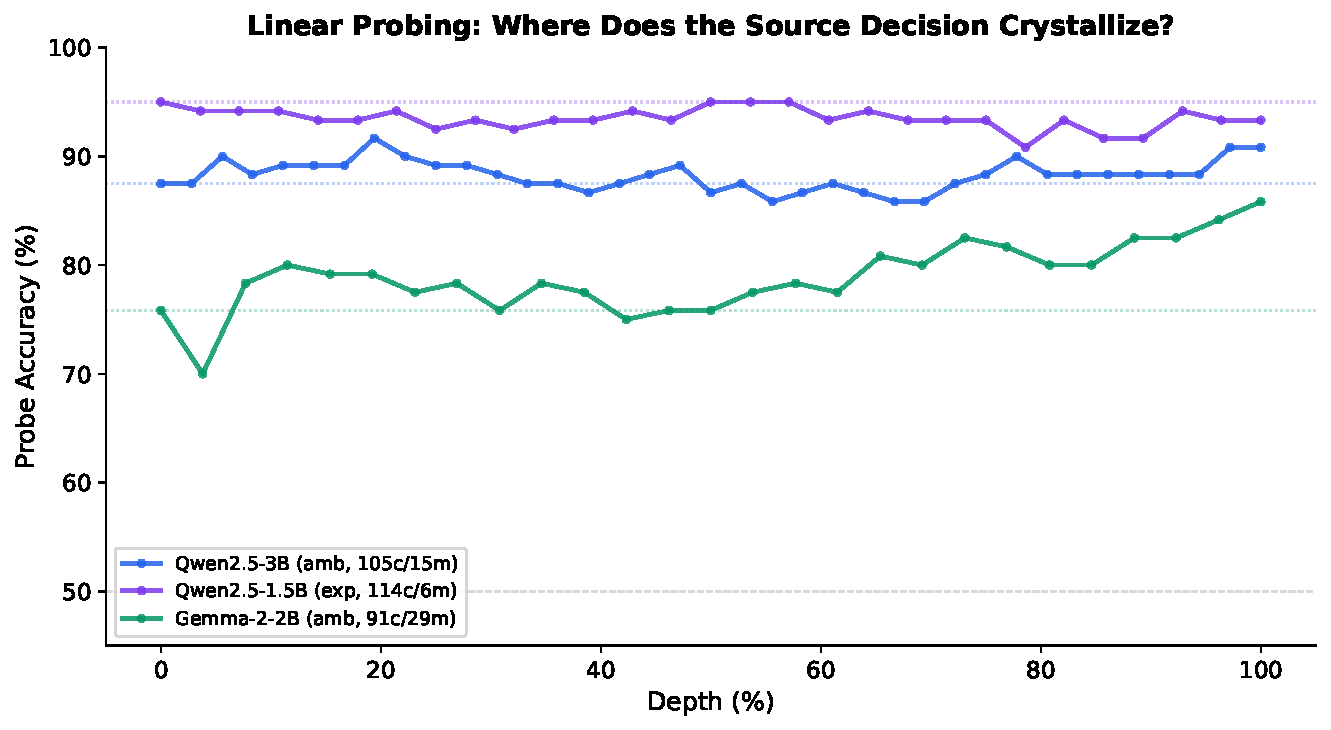
\includegraphics[width=\textwidth]{figures/fig5_probing.pdf}
        \caption{Linear probing: accuracy rises at circuit depth.}
        \label{fig:probing}
    \end{subfigure}
    \hfill
    \begin{subfigure}[b]{0.48\textwidth}
        \centering
        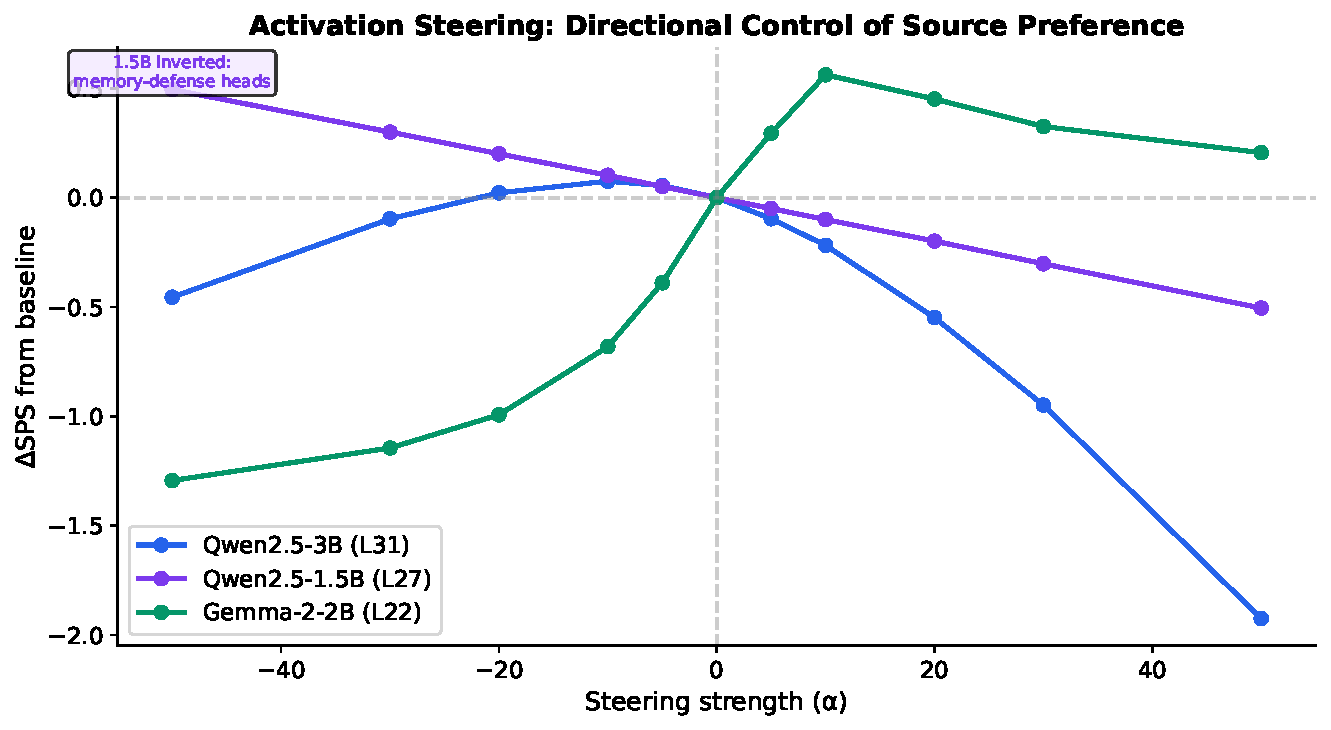
\includegraphics[width=\textwidth]{figures/fig4_steering.pdf}
        \caption{Steering: note Qwen-1.5B's inverted response.}
        \label{fig:steering}
    \end{subfigure}
    \caption{\textbf{Probing and Steering.} (a) Linear probes on residual stream activations show Gemma's clearest crystallization (15.8pp gain at L18--L22), aligning with causal patching. (b) Activation steering is directionally consistent with head polarity: Qwen-1.5B's inverted response is consistent with memory-defense heads, though CIs are wide.}
    \label{fig:probe_steer}
\end{figure*}

\begin{table}[t]
\centering
\resizebox{\columnwidth}{!}{%
\begin{tabular}{lccc}
\toprule
\textbf{Metric} & \textbf{Qwen-3B} & \textbf{Qwen-1.5B} & \textbf{Gemma-2B} \\
\midrule
Target layer & L31 & L27 & L22 \\
$\Delta$SPS ($\alpha{=}{-}50$) & $-0.46 \pm 2.10$ & $+0.49 \pm 1.21$ & $-1.29 \pm 0.90$ \\
Direction & Normal & \textbf{Inverted} & Normal \\
\midrule
Probe regime & Ambiguous & Explicit & Ambiguous \\
Probe gain & 5.8pp & 4.2pp & 15.8pp \\
\bottomrule
\end{tabular}%
}
\caption{Steering and probing results (95\% CI margins for $\Delta$SPS). Qwen-1.5B's inverted steering is directionally consistent with the memory-defense interpretation. Gemma's CI excludes zero. Wide Qwen CIs reflect high per-pair variance.}
\label{tab:steering_probe}
\end{table}


\textbf{Finding 7: Probe crystallization aligns with causal patching.} In Gemma, probe accuracy rises from 70\% to 86\% at L18--L22 (Figure~\ref{fig:probing}), precisely matching the residual patching circuit. Qwen models show weaker probing signal due to class imbalance (Table~\ref{tab:steering_probe}).

\textbf{Finding 8: Inverted steering is directionally consistent with memory-defense heads.} Qwen-1.5B's steering response is the mirror image of other models (Figure~\ref{fig:steering}): subtracting the ``context direction'' \emph{increases} context preference ($\Delta\text{SPS} = +0.49 \pm 1.21$ at $\alpha{=}{-}50$). The direction of the effect is consistent with the memory-defense interpretation, though the wide confidence interval includes zero. Three lines of evidence point in the same direction: DLA polarity, head patching sign, and steering direction.

\subsection{Cumulative Head-Set Patching}

To assess whether context-override is concentrated in a small set of heads rather than diffusely distributed, we measure the cumulative $\Delta$SPS from patching increasingly large head sets (Table~\ref{tab:cumulative}).

\begin{table}[t]
\centering
\resizebox{\columnwidth}{!}{%
\begin{tabular}{lccc}
\toprule
\textbf{Head set} & \textbf{Qwen-3B} & \textbf{Qwen-1.5B} & \textbf{Gemma-2B} \\
\midrule
Top-1 & $-0.25$ {\tiny $[\pm0.13]$} & $-0.12$ {\tiny $[\pm0.05]$} & $-0.25$ {\tiny $[\pm0.07]$} \\
Top-3 & $-0.74$ {\tiny $[\pm0.21]$} & $-0.36$ {\tiny $[\pm0.08]$} & $-0.70$ {\tiny $[\pm0.11]$} \\
Top-5 & $-1.17$ {\tiny $[\pm0.27]$} & $-0.34$ {\tiny $[\pm0.11]$} & $-0.98$ {\tiny $[\pm0.13]$} \\
Top-10 & $-2.09$ {\tiny $[\pm0.34]$} & $-0.46$ {\tiny $[\pm0.15]$} & $-1.54$ {\tiny $[\pm0.17]$} \\
\midrule
Rand-3 (late) & $-0.07$ {\tiny $[\pm0.22]$} & $+0.00$ {\tiny $[\pm0.07]$} & $-0.14$ {\tiny $[\pm0.09]$} \\
\bottomrule
\end{tabular}%
}
\caption{Cumulative head-set patching ($\Delta$SPS, additive approx.). Top-$k$ candidate heads monotonically increase, far exceeding random late-layer controls. 95\% CIs in brackets.}
\label{tab:cumulative}
\end{table}


\textbf{Finding 9: Candidate heads account for a substantial and highly non-random fraction of the head-level effect.} In Qwen-3B, the top-10 candidate heads produce $\Delta\text{SPS} = -2.09$ $[-2.43, -1.75]$, while a size-matched set of random late-layer heads produces only $-0.07$ $[-0.29, +0.16]$---a 30$\times$ difference. Similar separations hold for Qwen-1.5B ($-0.46$ vs $0.00$) and Gemma ($-1.54$ vs $-0.14$). The monotonic increase from top-1 to top-10 indicates that additional candidate heads contribute incrementally rather than redundantly. Note that the full residual-stream patching effect (Table~\ref{tab:patching}, $\Delta\text{SPS} \approx -13$) is larger, reflecting contributions from MLPs and head interactions not captured by additive head-level patching.

% ============================================================
% 5. DISCUSSION
% ============================================================
\section{Discussion}
\label{sec:discussion}

\subsection{Three Strategies for a Similar Function}

Our cross-model analysis suggests three distinct architectural strategies for source arbitration:

\textbf{Strategy 1---Concentrated Override (Qwen-3B):} A small number of heads at L31--L33 directly promote the context answer. Twenty significant heads, but 3--5 heads with high DLA ($> 0.2$) carry most of the attribution. No organized memory-defense counter-circuit was observed.

\textbf{Strategy 2---Memory Defense (Qwen-1.5B):} A dual-direction circuit: some heads promote context (positive DLA) while others actively defend memory (negative DLA). The net effect favors context (95.8\%), but reveals an internal tug-of-war. This may reflect weaker instruction-following capacity requiring explicit memory suppression.

\textbf{Strategy 3---Distributed Committee (Gemma-2B):} Many heads with individually modest contributions (top DLA $= 0.171$ vs Qwen's $0.324$). No single dominant head. Produces the clearest probing crystallization and the most monotonic steering response among the tested models.

\subsection{The Instruction-Reader Paradox}

A notable observation is that context-override heads do not attend to the document. This contrasts with the intuitive model of RAG as ``the model reads the document and extracts the answer.'' The mechanistic picture suggested by our experiments is:
\begin{enumerate}
    \item Early layers encode document content into distributed residual stream representations.
    \item Late-layer heads read the instruction to determine \emph{policy}.
    \item These heads write the appropriate answer, accessing document information through the residual stream---not through direct attention.
\end{enumerate}

\subsection{Implications for RAG Faithfulness}

Our findings suggest three practical implications:
\begin{enumerate}
    \item \textbf{Strengthen instruction signals}, not document signals---since the circuit reads instructions, not documents.
    \item \textbf{Use model-specific strategies}---a one-size-fits-all intervention is unlikely to work across architectures with fundamentally different strategies.
    \item \textbf{Monitor memory-defense pathways}---in smaller models, faithfulness failures may arise from memory defense being too strong, not context promotion being too weak.
\end{enumerate}

% ============================================================
% 6. LIMITATIONS
% ============================================================
\section{Limitations}
\label{sec:limits}

\begin{enumerate}
    \item \textbf{Synthetic benchmark:} Our facts and counterfactuals are constructed, not naturally occurring. Naturalistic RAG evaluation remains future work.
    \item \textbf{Small models:} We study 1.5B--3B parameter models. Larger models may implement qualitatively different circuits.
    \item \textbf{Single-token restriction:} Causal tracing is limited to single-token answers, covering 38--49\% of our dataset.
    \item \textbf{Steering ceiling:} Single-layer steering shifts SPS by 0.5--1.9 points, insufficient to flip strong context-following pairs (SPS $\approx$ 6--8). Multi-layer steering may be required.
    \item \textbf{Static conflicts:} We test factual substitution only. Conflicts involving reasoning, temporal changes, or partial contradictions are not covered.
\end{enumerate}

% ============================================================
% 7. CONCLUSION
% ============================================================
\section{Conclusion}
\label{sec:conclusion}

We present a mechanistic investigation of source arbitration in instruction-tuned language models. Through six complementary causal interventions across three models from two families, we identify a compact late-layer circuit (final 8--12\% of depth) whose heads function as instruction readers, not document copiers. We observe three distinct architectural strategies---concentrated override, memory defense, and distributed committee---providing suggestive evidence of a recurring functional role for late-layer source-arbitration heads across the tested models. These findings suggest that RAG faithfulness may be better understood as an instruction-processing problem rather than a document-attention problem, with potential implications for the design of more faithful retrieval-augmented systems.

% ============================================================
% 8. CROSS-MODEL SUMMARY (DASHBOARD)
% ============================================================
\section*{Acknowledgments}
Redacted for double-blind review.

\bibliographystyle{icml2026}
\bibliography{bib/references}

% ============================================================
% APPENDIX
% ============================================================
\appendix
\onecolumn

\section{Cross-Model Summary Dashboard}
\label{app:dashboard}

\begin{figure}[htbp]
    \centering
    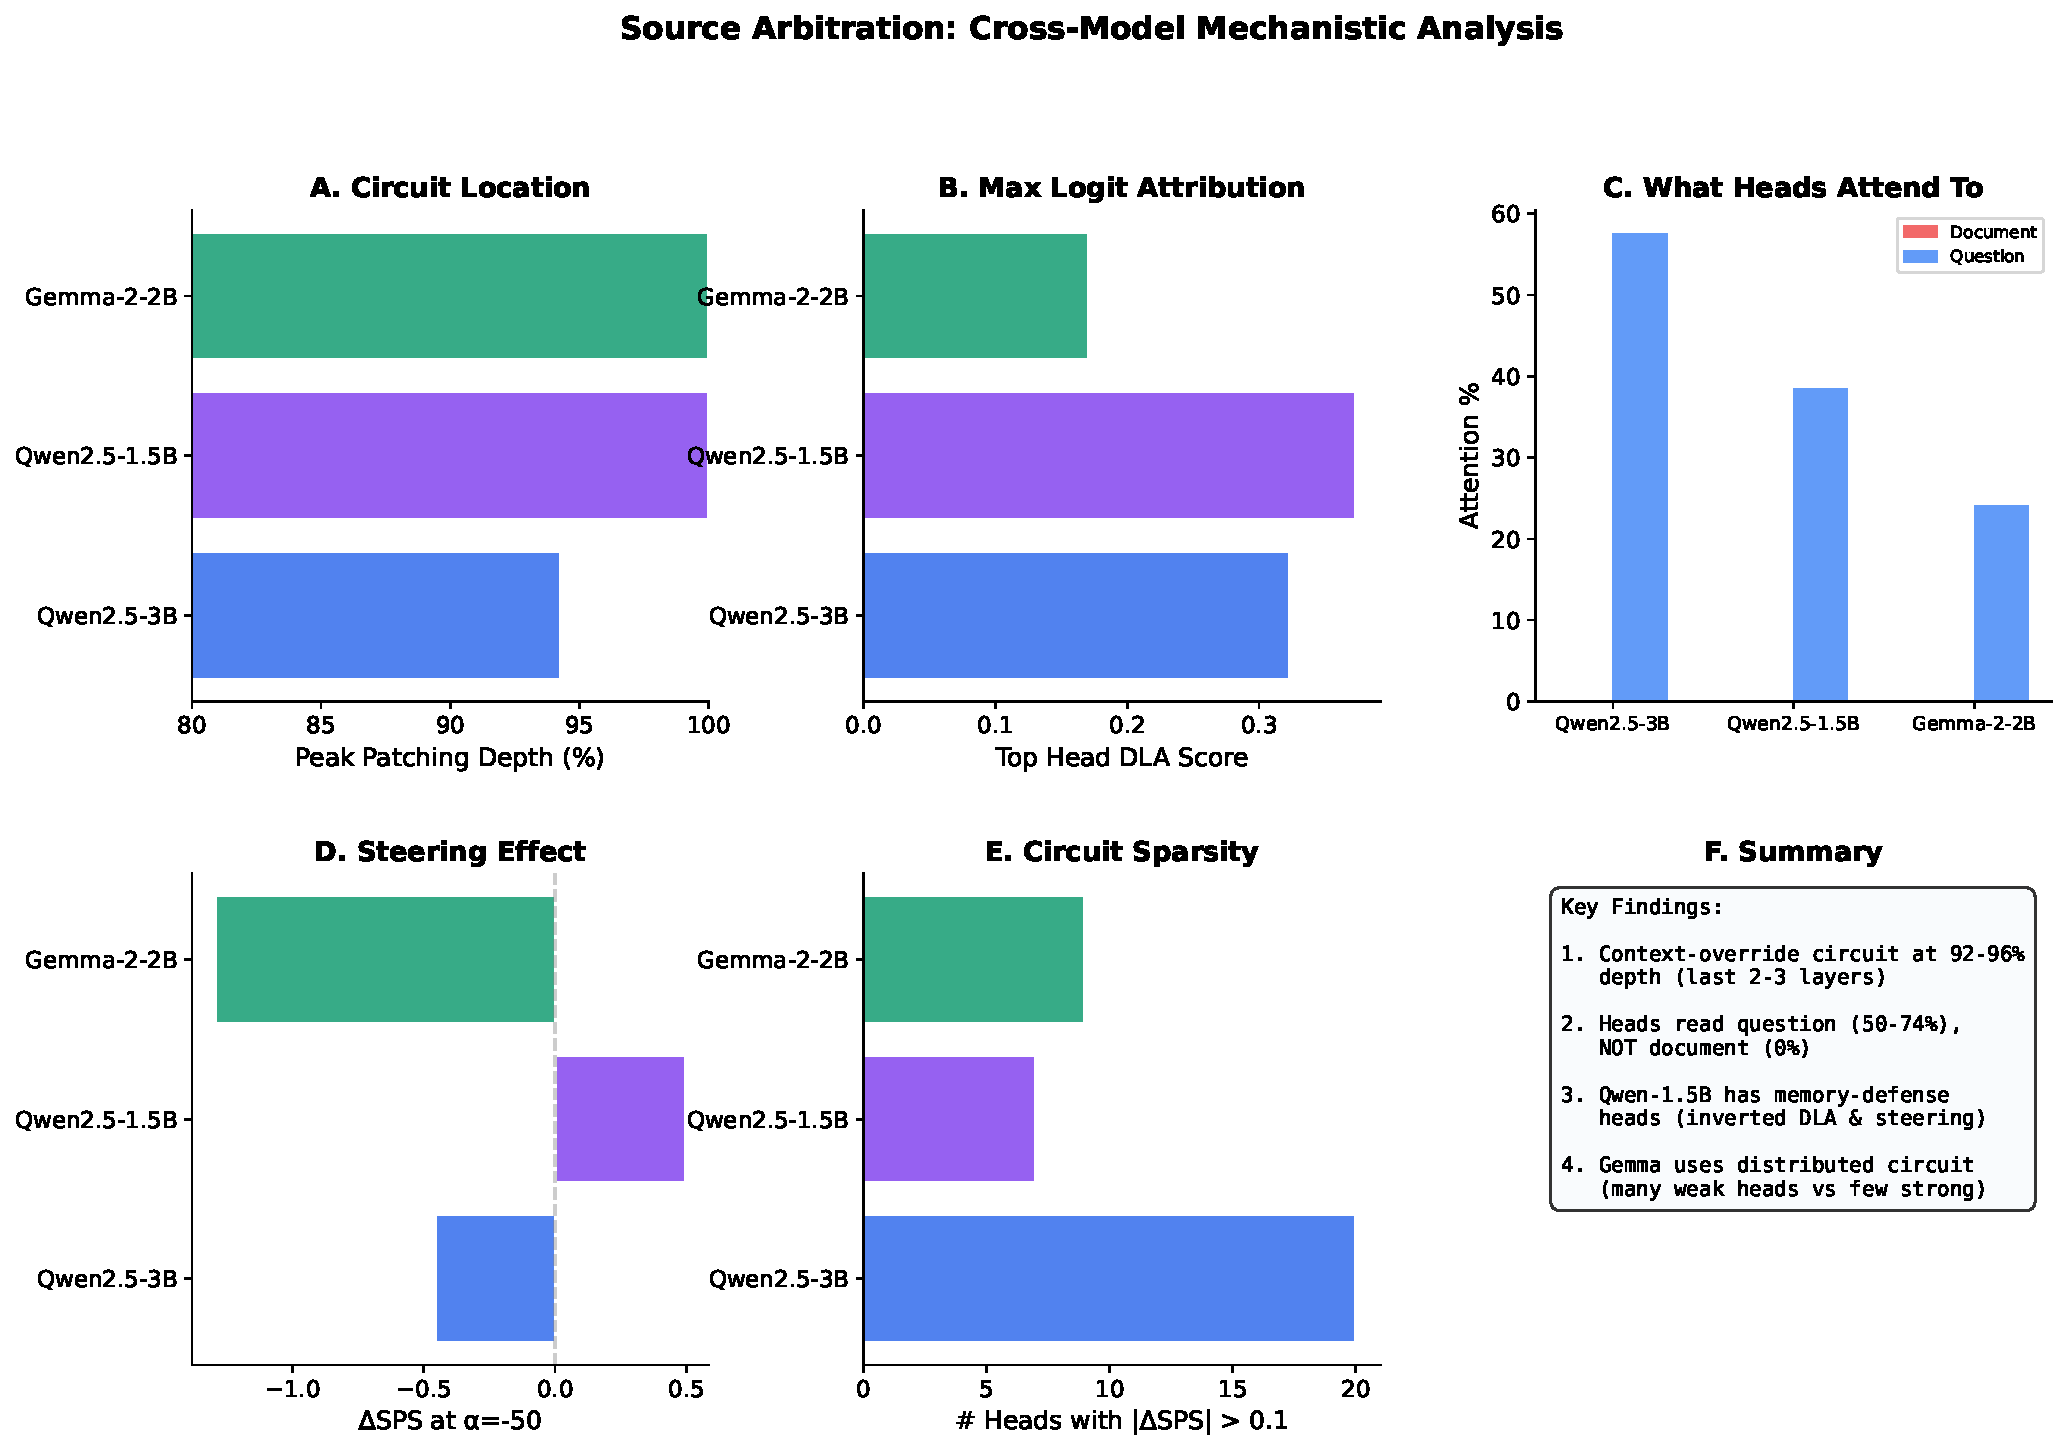
\includegraphics[width=0.9\textwidth]{figures/fig6_summary_dashboard.pdf}
    \caption{\textbf{Cross-Model Summary Dashboard.} Six-panel comparison: (A) circuit location, (B) max DLA score, (C) attention targets, (D) steering effect, (E) circuit sparsity, and (F) key findings summary.}
    \label{fig:dashboard}
\end{figure}

\section{Dataset Construction}
\label{app:dataset}

The benchmark evaluates source preference under direct conflict. We generate 501 factual tuples across categories including geography, science, history, and culture. Each tuple pairs a real-world fact with a plausible counterfactual distractor.

\paragraph{Prompt templates.} For explicit context: \textit{``Document: \{document with counterfactual\}. Question: Based only on the document above, \{question\}.''}  For ambiguous: the same document but without explicit source instruction. For explicit memory: \textit{``Using your own knowledge (not the document), \{question\}.''}

\paragraph{Token-variant scoring.} Modern tokenizers are context-sensitive. ``Rome'' may map to distinct tokens depending on preceding whitespace. We generate a pool of single-token variants for both answers:
\begin{equation}
\text{SPS}(S) = \max_{t \in T_{\text{ctx}}} L_S(t) - \max_{t \in T_{\text{mem}}} L_S(t)
\end{equation}
Filtering requires both answers to have valid single-token representations and sufficient logit margin.

\section{Intervention Protocol Details}
\label{app:intervention}

We define three runs for each intervention:
\begin{itemize}
    \item \textbf{Clean Run:} Standard forward pass on the target prompt.
    \item \textbf{Corrupted Run:} Forward pass where the document is removed (no-document baseline).
    \item \textbf{Patched Run:} Corrupted run where specific activations are replaced with cached clean-run values.
\end{itemize}

For head patching, we replace individual head outputs (\texttt{hook\_z}) at the answer position. For residual patching, we replace the full residual stream at layer $\ell$.

\section{Evidence Ladder}
\label{app:evidence}

We separate claims by evidential strength:
\begin{itemize}
    \item \textbf{Sufficiency:} Activation patching---restoring clean activations recovers $\Delta$SPS.
    \item \textbf{Necessity:} Head ablation---zeroing heads reduces context-preference margin.
    \item \textbf{Mechanistic:} DLA and attention decomposition---what heads write and read.
    \item \textbf{Causal sufficiency:} Activation steering---adding direction vectors shifts behavior.
    \item \textbf{Information-theoretic:} Linear probing---when does information crystallize.
\end{itemize}

\section{Detailed Probing Results}
\label{app:probing}

The logistic regression probe is trained at each layer on residual stream activations to predict context vs.\ memory following. For Gemma-2B in the ambiguous regime (91 context, 29 memory examples), probe accuracy rises from 70.0\% (layer 0) to 85.8\% (layer 25), a 15.8 percentage point gain. The steepest increase occurs at L18--L22, matching the residual patching circuit exactly.

For Qwen-3B (105 context, 15 memory), the majority-class baseline is 87.5\%, and the probe hovers at 86--92\%---insufficient variance for clean signal. For Qwen-1.5B (114 context, 6 memory), the baseline is 95\%, leaving probing uninformative.

\section{Steering Protocol}
\label{app:steering}

We compute the context direction as:
\begin{equation}
d = \mathbb{E}[\text{attn\_out}_{\text{ctx-win}}] - \mathbb{E}[\text{attn\_out}_{\text{mem-win}}]
\end{equation}
at the peak patching layer. During inference, we add $\alpha \times d$ to the attention output. We sweep $\alpha \in \{-50, -30, -20, -10, -5, 0, 5, 10, 20, 30, 50\}$.

Key results:
\begin{itemize}
    \item \textbf{Qwen-3B (L31):} $\Delta$SPS ranges from $-0.46$ (at $\alpha{=}{-}50$) to $-1.92$ (at $\alpha{=}50$). Normal direction but overshoots at large positive $\alpha$.
    \item \textbf{Qwen-1.5B (L27):} Inverted. $\Delta$SPS $= +0.49$ at $\alpha{=}{-}50$, $-0.50$ at $\alpha{=}50$. The ``context direction'' at L27 actually points \emph{away} from context because the dominant heads are memory-defense heads.
    \item \textbf{Gemma-2B (L22):} Cleanest response. $\Delta$SPS $= -1.29$ at $\alpha{=}{-}50$, $+0.30$ at $\alpha{=}10$, then saturation. Monotonic in the useful range.
\end{itemize}

\section{Reproducibility}
\label{app:reproduce}

\subsection{Environment and Compute}

All experiments were conducted using Python~3.11, PyTorch~2.11, and Transformers~5.8 on consumer-grade hardware with MPS acceleration. Models are loaded from HuggingFace Hub without fine-tuning. The full pipeline (3 models $\times$ 6 interventions) requires approximately 5.5~hours of wall-clock time. All scripts use a fixed random seed (\texttt{seed=42}) and sample \texttt{max\_pairs=40} matched pairs per experiment. Code and data are available in the supplementary material.

\subsection{Pipeline Summary}

The experimental pipeline consists of 14 scripts executed sequentially:
\begin{enumerate}
    \item \textbf{Dataset} (Scripts 00--04): Generate 501 facts, validate token variants, compute baselines, construct matched pairs, lock model configs.
    \item \textbf{Causal tracing} (Scripts 05--06): Residual stream patching and head patching across target layers.
    \item \textbf{Mechanistic analysis} (Scripts 08--09): Attention pattern decomposition and Direct Logit Attribution.
    \item \textbf{Verification} (Scripts 10--11): Linear probing and activation steering.
    \item \textbf{Synthesis} (Scripts 12--14): Figure generation, cross-model comparison, cumulative ablation, and bootstrap CIs.
\end{enumerate}

\subsection{Expected Metric Ranges}

Table~\ref{tab:reproduce} provides expected ranges for key metrics. Minor numerical differences ($\pm5\%$) are expected due to floating-point non-determinism across hardware backends.

\begin{table}[htbp]
\centering
\small
\begin{tabular}{lcc}
\toprule
\textbf{Metric} & \textbf{Expected} & \textbf{Range} \\
\midrule
Peak layer depth & 88--100\% & $\pm 5\%$ \\
Peak $\Delta$SPS & $-11$ to $-14$ & $\pm 30\%$ \\
Top DLA & 0.17--0.37 & $\pm 40\%$ \\
Doc attention & 0.0\% & Exact \\
1.5B steer inversion & $\Delta$SPS $> 0$ & Qualitative \\
\bottomrule
\end{tabular}
\caption{Expected metric ranges for reproduction. ``Exact'' indicates the finding should hold regardless of seed. ``Qualitative'' indicates the sign should be consistent.}
\label{tab:reproduce}
\end{table}

\subsection{Variability Sources}

Three factors contribute to numerical variability: (1)~\textbf{Hardware backend}: MPS and CUDA produce slightly different float32 results; (2)~\textbf{Pair sampling}: with \texttt{max\_pairs=40}, different seeds select different fact subsets---qualitative findings (late-layer localization, 0\% document attention, 1.5B inversion) are robust across seeds; (3)~\textbf{Model versioning}: HuggingFace model weights may be updated; we recommend pinning to specific commit hashes for exact reproduction.

\end{document}
